\chapter{Problem Solving}

Having described the problem at hand as well as relevant deep learning methods it is time to join it all into one single method. In this chapter we will cover a detailed explanation of the method proposed, the metrics that will be used to compare across architectures and hyperparameters, the experiments carried out to show its usefulness and the results obtained.

\section{Method description}\label{sec:descr}

I have described how the cell classification problem was tackled with the help of convolutional neural networks. I have also explained two algorithms used for node classification. It is time to merge both fields. For that, we need to describe the cell classification problem as a node classification problem. As mentioned in \autoref{sec:gnn}, the nodes of our graph are going to be the individual cells. It is left to define the edges. We are going to consider two nodes (cells) to be related if they are sufficiently close. By sufficiently close it is meant that their euclidean distance is less than some previously defined amount. Apart from that, to have manageable graphs, the degree of each node is limited by only considering a small amount of nearby nodes as possible connections. This way we ensure the number of edges increases linearly with the number of nodes making our method more scalable. An example of such graph is on \autoref{fig:graph_def}. 

\begin{figure}[h]
    \centering
    \begin{subfigure}{0.3\textwidth}
      \centering
      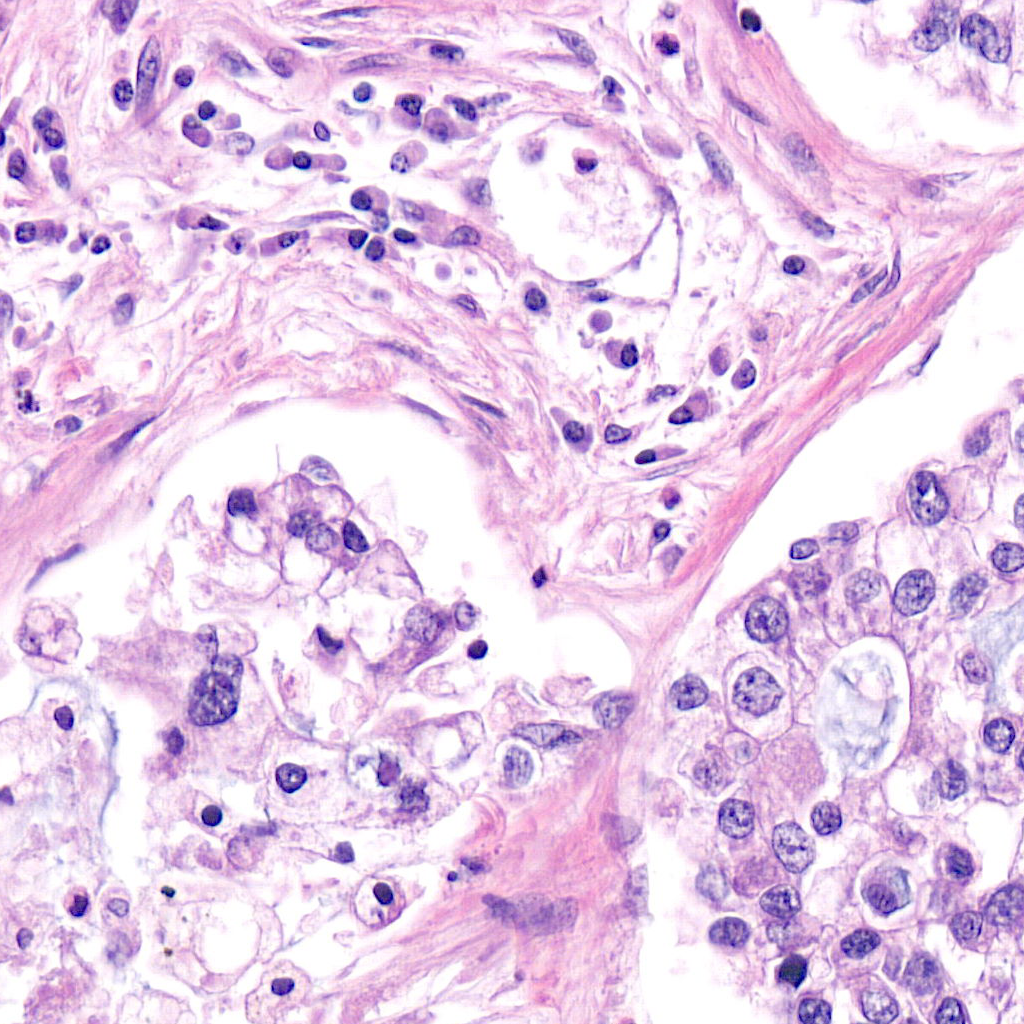
\includegraphics[width=\textwidth]{imgs/img_ex.png}
    \end{subfigure}
    \begin{subfigure}{0.3\textwidth}
      \centering
      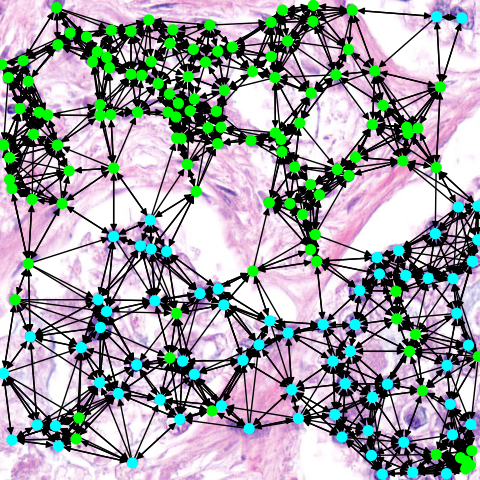
\includegraphics[width=\textwidth]{imgs/graph_overlay.png}
    \end{subfigure}
    \begin{subfigure}{0.3\textwidth}
      \centering
      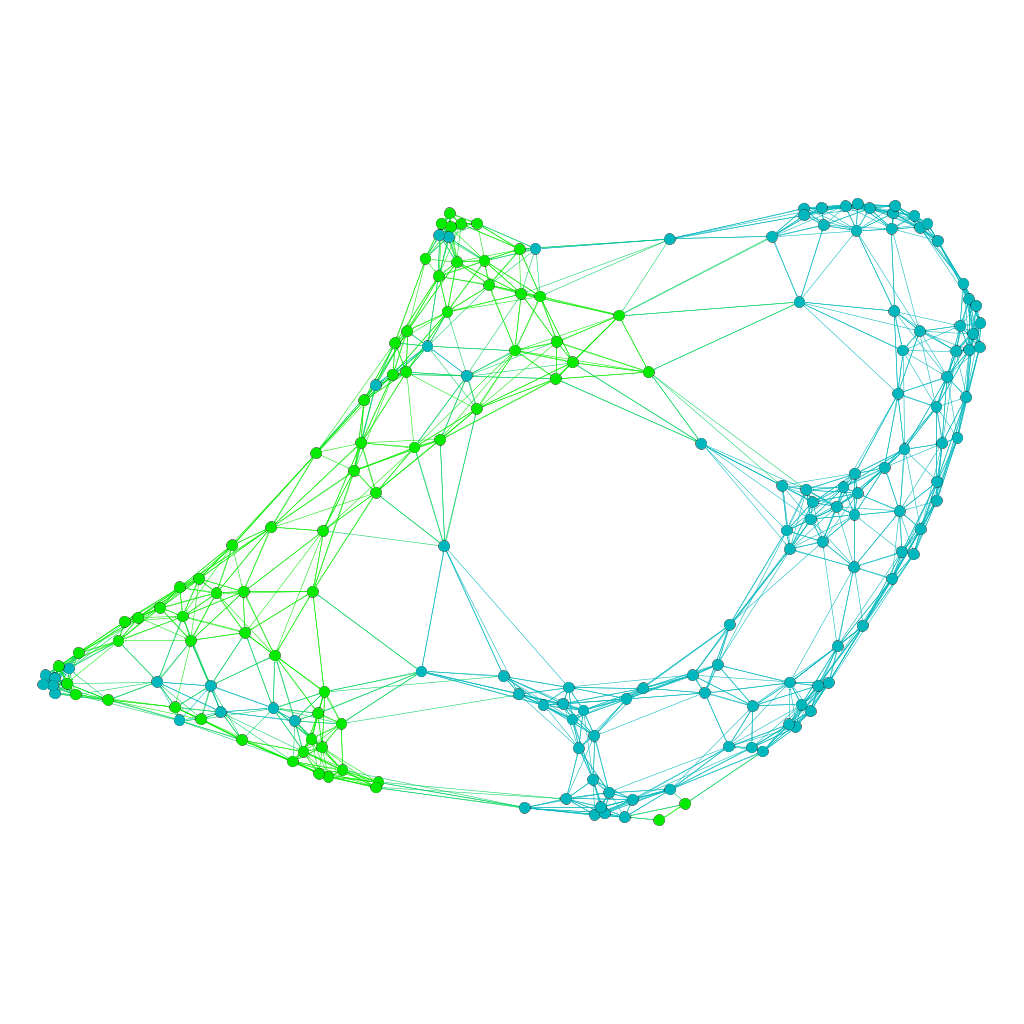
\includegraphics[width=\textwidth]{imgs/graph_class.png}
    \end{subfigure}
    \caption{Example of an image and its associated graph. At the middle we have the nodes located at their corresponding centroids. However, a graph is an abstraction, so it may also be viewed as in the right image, since it only encodes relationships, not absolute positions. The visualization of the graph was made using Gephi \cite{gephi}.}
    \label{fig:graph_def}
\end{figure}

Given nodes and edges we can still give more information to the graph neural network. In \autoref{sec:gcn} we showed that the network can be given an initial set of features $\bh_k^{(0)}$. Those features can be anything that gives information about the cell. We decided to use the following set of descriptive features:

\begin{itemize}
    \item The area and perimeter of the cell measured in pixels. Those values should give information about the shape of the cell.
    \item The standard deviation of the values of the pixels in gray format. This magnitude is supposed to bring insights about the luminosity of the cell.
    \item The histogram of the red, green and blue colour channels. We expect it to summarise the information about the colour of the cell.
    \item A prior distribution of the class. It is computed using the output of Hovernet. Each class probability is inferred as the number of pixels of that class predicted by Hovernet divided by the total number of pixels of the cell.
\end{itemize}

\noindent Later on, in \autoref{sec:exp} an experiment is made to discover how relevant the selected features are.

\section{Evaluation metrics}\label{sec:metrics}

This section is going to provide a review of the most common metrics for any classification problem, either binary of multiclass. 

\subsection{Confusion Matrix}

Prior to defining any metric we have to define the concept of confusion matrix. Most of the metrics described can be expressed in terms of it. The confusion matrix is a way of measuring how precise is any method. For a binary classification problem one has positive (1) and negative (0) classes. If the model correctly predicts the positive or negative class it is called true positive and true negative. Then, if the model incorrectly predicts positive it is called false positive and if it infers negative wrongly it is denoted by false negative. Confusion matrices are typically expressed as shown below.

\begin{table}[ht]
\centering
\caption{Binary confusion matrix.}
\begin{tabular}{c c c|c|}
& & \multicolumn{2}{c}{\textbf{Predicted}} \\ \cline{3-4}
& & \multicolumn{1}{|c|}{Positive} & Negative \\ \cline{2-4}
\multirow{2}{*}{\textbf{Actual}} & \multicolumn{1}{|c|}{Positive} & $TP$ & $FP$ \\ \cline{2-4}
                     & \multicolumn{1}{|c|}{Negative} & $FN$ & $TN$ \\ \cline{2-4}
\end{tabular}
\label{table:confusion_matrix}
\end{table}

For more than two classes sometimes an adaptation is made. Instead of adding more rows and columns the matrix is built considering one class against all the others. In that case several confusion matrices are needed. Of course, one can also create a bigger confusion matrix as follows

\begin{table}[ht]
\centering
\caption{Multi-class confusion matrix. Here the terms true positive, negative and false positive, negative lack any meaning unless you consider one class against the others.}
\label{table:confusion_matrix2}
\begin{tabular}{c c c|c|c|c|c|}
& & \multicolumn{5}{c}{\textbf{Predicted}} \\ \cline{3-7}
& & \multicolumn{1}{|c|}{Class 1} & Class 2 & Class 3 & Class 4 & Class 5 \\ \cline{2-7}
\multirow{5}{*}{\textbf{Actual}} & \multicolumn{1}{|c|}{Class 1} & & & & & \\ \cline{2-7}
                     & \multicolumn{1}{|c|}{Class 2} & & & & & \\ \cline{2-7}
                     & \multicolumn{1}{|c|}{Class 3} & & & & & \\ \cline{2-7}
                     & \multicolumn{1}{|c|}{Class 4} & & & & & \\ \cline{2-7}
                     & \multicolumn{1}{|c|}{Class 5} & & & & & \\ \cline{2-7}
\end{tabular}
\end{table}

\subsection{Accuracy}\label{sec:acc}

The first metric we will be defining is the most intuitive one. It is basically the percentage of correct predictions. Using the terminology from \autoref{table:confusion_matrix} it can be expressed as 
\begin{equation}
    \frac{TP + TN}{TP + FP + TN + FN}
\end{equation}

The main disadvantage of the accuracy comes when dealing with imbalanced datasets. By predicting the class that appears the most a high accuracy can be easily achieved in those cases.

The accuracy is a binary classification metric, later on in \autoref{sec:micro} an adaptation to multi-class problems is described.

\subsection{Precision}

The accuracy requires to know how many true negatives there are. But in some problems like object detection that is not always possible. Due to how labels are constructed in some cases it is impossible to know how many true negatives can be considered, although in the case of object detection the trend seems to be changing these days \cite{kirillov2023segment}. In those cases it makes sense to define the percentage of correct predictions only within the positive class. Mathematically, precision is defined as

\begin{equation}
    P = \frac{TP}{TP + FP}
\end{equation}

This metric, however, can be easily fooled. In an image with hundreds of cells, by only predicting one true tumoural cell you achieve a precision of $100\%$. But that is a useless value since you would be missing on most relevant cells.

\subsection{Recall}

As opposed to precision, recall focuses more on what relevant values are retrieved rather than them being correct. It is defined like this

\begin{equation}
    R = \frac{TP}{TP + FN}
\end{equation}

Again, this metric can also be fooled. By predicting everything as positive you achieve $100\%$. Since this metric ignores false positives you are left with a biased metric against the negative label.

\subsection{$F_1$ Score}\label{sec:f1}

In order to take the best from precision and recall, the F-measure was proposed in 1992 at the Proceedings of the 4th conference on Message understanding \cite{10.5555/1072064}. The F-measure is defined as the harmonic mean between precision and recall.

\begin{equation}
    \frac{2 \cdot P \cdot R}{P + R} = \frac{2 \cdot TP}{2 \cdot TP + FP + FN}
\end{equation}

Nowadays it is called $F_1$ score because that measure has been extended to what is called the $F_\beta$ score.

\begin{equation}
    F_\beta = \frac{(1+\beta^2) \cdot P \cdot R}{\beta^2 \cdot P + R} = \frac{(1+\beta^2) \cdot TP}{(1+\beta^2) \cdot TP + \beta^2 \cdot FP + FN}
\end{equation}

\noindent By taking $\beta=1$ the original F-measure is obtained. This metric achieves $100\%$ when all the relevant positive samples are retrieved and only the relevant samples, therefore it is not so easily fooled. Moreover, it is less prone to suffer from class imbalance as the accuracy does.

There are three ways of extending the $F_1$ score to a multi-class classification problem. All of them involve some kind of averaging the individual $F_1$ scores computed by considering one class against all the others. 

\subsection{Macro $F_1$ Score}

The first way of averaging individual $F_1$ scores is by simply taking the arithmetic mean. If we have $n$ classes, and we call $F_1^i$ the $F_1$ score of the class $i$ against the others, then the macro $F_1$ score is

\begin{equation}
    \frac{1}{n} \sum_{i=1}^n F_1^i
\end{equation}

The main drawback of only considering this metric is that classes can be imbalanced. In fact, for multi-class problems that is the rule rather than the exception. Giving equal weights to all of the classes harms the less represented labels.

\subsection{Weighted $F_1$ Score}

As a way of solving the main drawback of the macro $F_1$ score one can deal with the weighted $F_1$ score that averages individual scores based on their support, that is, based on the number of true instances by class. Let's call $n_i$ the number of true instances of class $i$, then the weighted $F_1$ score is

\begin{equation}
    \sum_{i=1}^n \frac{n_i \cdot F_1^i}{n_1 + \dots + n_n}
\end{equation}

\subsection{Micro $F_1$ Score}\label{sec:micro}

Another way of averaging the individual $F_1$ scores is by micro-averaging. When macro-averaging, true positives, false negatives and false positives are computed per-class prior to averaging all the scores computed as defined in \autoref{sec:f1}. Micro-averaging changes the order. True positives, false negatives and false positives are first aggregated among all the classes and then the micro $F_1$ score is computed using the formula in \autoref{sec:f1}. To illustrate the computation let's consider the matrix from \autoref{table:confusion_matrix2} and let's also fill it with false positives / negatives and true positives, giving the matrix in \autoref{table:confusion_matrix3}. Now, this terminology only makes sense when splitting by class. For that reason we will denote by $TP_i$ the true positives of class $i$, and $FP_i$, $FN_i$ the false positives and negatives of same class $i$. Notice that what is a false positive for one class can be a false negative for another.

\begin{table}[ht]
\centering
\caption{Multi-class confusion matrix. The values in the diagonal are all true positives when considering one class agains the others. Depending on which class you are considering, the values considered false positives and false negatives could be interchanged.}
\begin{tabular}{c c c|c|c|c|c|}
& & \multicolumn{5}{c}{\textbf{Predicted}} \\ \cline{3-7}
& & \multicolumn{1}{|c|}{Class 1} & Class 2 & Class 3 & Class 4 & Class 5 \\ \cline{2-7}
\multirow{5}{*}{\textbf{Actual}} 
 & \multicolumn{1}{|c|}{Class 1} & $TP_1$ & $FP_1$, $FN_2$ & $FP_1$, $FN_3$ & $FP_1$, $FN_4$ & $FP_1$, $FN_5$ \\ \cline{2-7}
 & \multicolumn{1}{|c|}{Class 2} & $FP_2$, $FN_1$ & $TP_2$ & $FP_2$, $FN_3$ & $FP_2$, $FN_4$ & $FP_2$, $FN_5$ \\ \cline{2-7}
 & \multicolumn{1}{|c|}{Class 3} & $FP_3$, $FN_1$ & $FP_3$, $FN_2$ & $TP_3$ & $FP_3$, $FN_4$ & $FP_3$, $FN_5$ \\ \cline{2-7}
 & \multicolumn{1}{|c|}{Class 4} & $FP_4$, $FN_1$ & $FP_4$, $FN_2$ & $FP_4$, $FN_3$ & $TP_4$ & $FP_4$, $FN_5$ \\ \cline{2-7}
 & \multicolumn{1}{|c|}{Class 5} & $FP_5$, $FN_1$ & $FP_5$, $FN_2$ & $FP_5$, $FN_3$ & $FP_5$, $FN_4$ & $TP_5$ \\ \cline{2-7}
\end{tabular}
\label{table:confusion_matrix3}
\end{table}

The micro-average is then the sum of the diagonal divided by the sum of all the entries in the matrix. It is quite similar to how the accuracy is computed. For that reason sometimes this metric is referred to as the accuracy in multi-class problems.

\newpage
\subsection{Dice's coefficient}

The Dice's coefficient can be viewed as a generalisation of the $F_1$ score. Given two sets $X$ and $Y$ the Dice's coefficient is defined as 

\begin{equation}
    \frac{2\cdot |X \cap Y|}{|X| + |Y|}
\end{equation}

If we consider $X$ as the set of relevant items and $Y$ as the set of retrieved elements, we obtain the $F_1$ score. To show that, let's see what are the sets of retrieved and relevant objects. The relevant items are the sum of true positives and false negatives. The retrieved ones are the sum of true positives and false positives. The intersection is clearly just the true positives, so $|X\cap Y| = TP$ and also $|X|+|Y|=2\cdot TP + FN + FP$. Substituting into the formula for the Dice's coefficient the formula for the $F_1$ score appears.

But the Dice's coefficient can be used for more than that. It can be used as a metric for image segmentation problems. By defining $X$ as the set of pixels that belongs to a class in the ground truth and $Y$ as the set of pixels of the same class but in the predictions, the Dice's coefficient can be used for evaluating the performance of a segmentation model. 

Furthermore, it is possible to extend that measure to a loss function. All the metrics presented so far require a thresholding function at the end. That function has a discontinuity at $0.5$ but worse than that, are completely flat in the rest of the $[0,1]$ interval, which means the gradient is zero. A null gradient stops any deep learning method from using them as loss functions. The adaptation of the Dice's coefficient to a loss was made by Milletari et al. \cite{milletari2016vnet}. The idea is to take advantage from the fact that pixel class probabilities range from 0 to 1. The Dice's coefficient can be seen as a boolean operation. Therefore, the Dice's loss is a function that when given just 0s and 1s is that same boolean operation, but is also defined in the rest of the $[0,1]$ interval and not just in the extremes. To be consistent with the original notation, let's call $p_i$ to the predicted probabilities and $g_i$ to the ground truth probabilities, where $i$ ranges from $1$ to $N$ being $N$ the total number of pixels. Thus, the Dice's loss is

\begin{equation}
    D = \frac{2 \sum_{i=1}^N p_i g_i}{\sum_{i=1}^N p_i^2 + \sum_{i=1}^N g_i^2}
\end{equation}

It is clear that when $p_i \in \{0,1\} \forall i$ and $g_i \in \{0,1\} \forall i$ the result is the same as the Dice's coefficient. But in this new version, the gradient can be computed with respect to any pixel with this formula.

\begin{equation}
    \frac{\partial D}{\partial p_j} = 2\cdot \frac{g_j\left(\sum_{i=1}^N p_i^2 + \sum_{i=1}^N g_i^2\right) - 2p_j \sum_{i=1}^N p_ig_i}{\left(\sum_{i=1}^N p_i^2 + \sum_{i=1}^N g_i^2 \right)^2}
\end{equation}

\subsection{ROC AUC}

Another metric that avoids thresholding the probabilities is the Receiver Operating Characteristic Area Under the Curve. It evaluates the ordering of the probabilities instead of the actual predictions. Before diving into the details of the ROC curve, we need to first define the false positive rate.

\begin{equation}
    FPR = \frac{FP}{FP + TN}
\end{equation}

False positives and true negatives depend on the threshold selected. Using $0.5$ gives some predictions while using $-1$ give everything as positive and using $2$ returns all negatives. By changing the threshold different FPR are obtained. Moreover, the Recall, also known as true positive rate (TPR), changes when using different thresholds too. There is a balance between both of them, similar to what happened with precision and recall. Both metrics can be fooled, but not at the same time. So by changing the threshold one can measure which metric is being fooled the most. The ROC curve plots the TPR in the y axis and the FPR in the x axis. An example is on \autoref{fig:auc}.

\begin{figure}[ht]
    \centering
    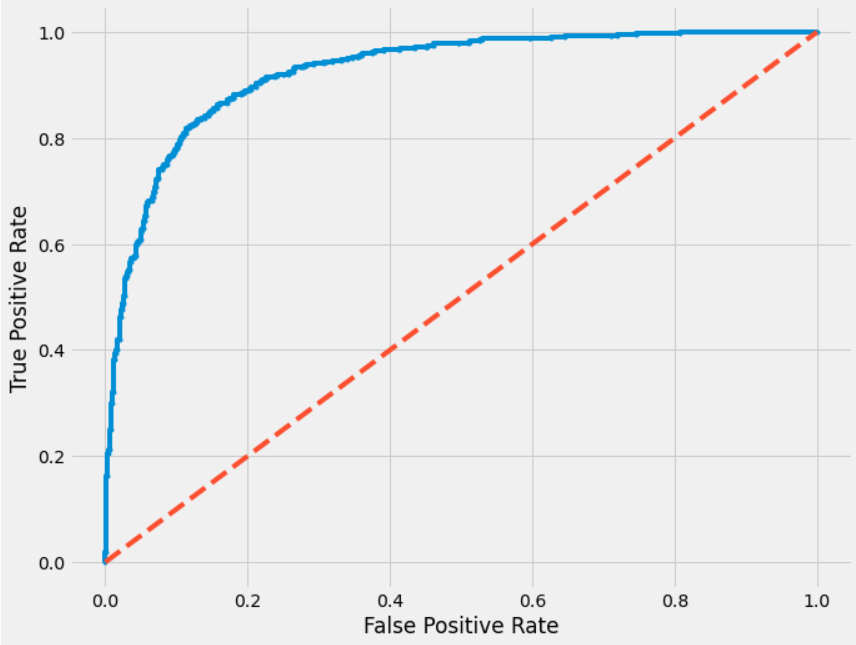
\includegraphics[width=\textwidth]{imgs/auc.png}
    \caption{Example of a ROC curve.}
    \label{fig:auc}
\end{figure}

This curve always starts in the $(0,0)$ and finishes in the $(1,1)$ corresponding to thresholds $2$ and $-1$ respectively (or any other threshold that returns all negatives and all positives). Given that, the ROC AUC is, as its name states, the area under that curve. A random classifier would yield the orange line in \autoref{fig:auc} that goes from $(0,0)$ to $(1,1)$, while a perfect classifier would go from $(0,0)$ to $(0,1)$ and then to $(1,1)$. Therefore, any classifier has an AUC roughly between $0.5$ and $1$. Notice that an AUC of $0$ corresponds to an adversarial classifier, which is a perfect classifier but changes negatives with positives.

\subsection{Calibration}

To finish this section, I'll cover a different way of evaluating classifiers. Normally, the effectiveness of a classifier is measured depending on how well it classifies samples. But that has its flaws too. It may be interesting to have a way of measuring the uncertainty of a prediction. If I am going to be diagnosed with cancer I want to know how likely that is wrong. Having a $51\%$ probability of dying is not the same as having a $99.9\%$ probability. None of the previous metrics evaluates the quality of the uncertainty provided by the probabilities. Deep learning methods oftentimes suffer from overconfidence \cite{wei2022mitigating, meronen2023fixing, melotti2022reducing}. Neural networks typically provide probabilities that are close to $1$ even when the available information is not enough to be so sure about that prediction. To analyse that phenomena, reliability diagrams were invented. An example is provided in \autoref{fig:rel}. On the x axis there is the predicted probability while in the y axis is an estimation of the real probability.

\begin{figure}[ht]
    \centering
    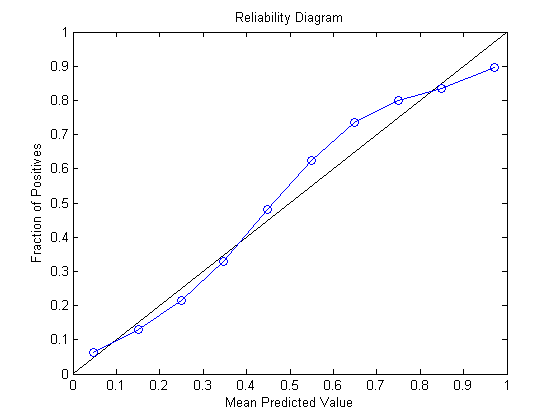
\includegraphics[width=\textwidth]{imgs/rel.png}
    \caption{Example of a reliability diagram.}
    \label{fig:rel}
\end{figure}

More specifically, predicted probability is quantised. The x axis represents the probability distribution of the model, but we only have a finite collection of samples, so that distribution is estimated using the histogram. This means that the points in \autoref{fig:rel} in fact represents a set of samples that are predicted with very similar probabilities. The magnitude in the y axis is how many of them really are positive. As an example, suppose we have 4 samples predicted with probabilities $0.74, 0.75, 0.75, 0.76$ and only three of them are real positives. The mean predicted probability of that group is $0.75$, and the real probability is also $0.75$ since 3 out of 4 are positives. This would give a point in the black line, a perfectly calibrated point. On the other hand, consider the following example. Four samples, 3 with probability 1 and 1 with probability 0. From the first three, one is negative and two are positive. The sample with probability 0 is negative. In this case, we have a point at $(0,0)$ and another at $(1,\frac{2}{3})$. This time, we have a less calibrated prediction. Nonetheless, in both examples we have an accuracy of $75\%$. This illustrates the fact that calibration is independent from how well you classify samples. An example of an uncalibrated model is on \autoref{fig:hov_rel}.

\begin{figure}[ht]
    \centering
    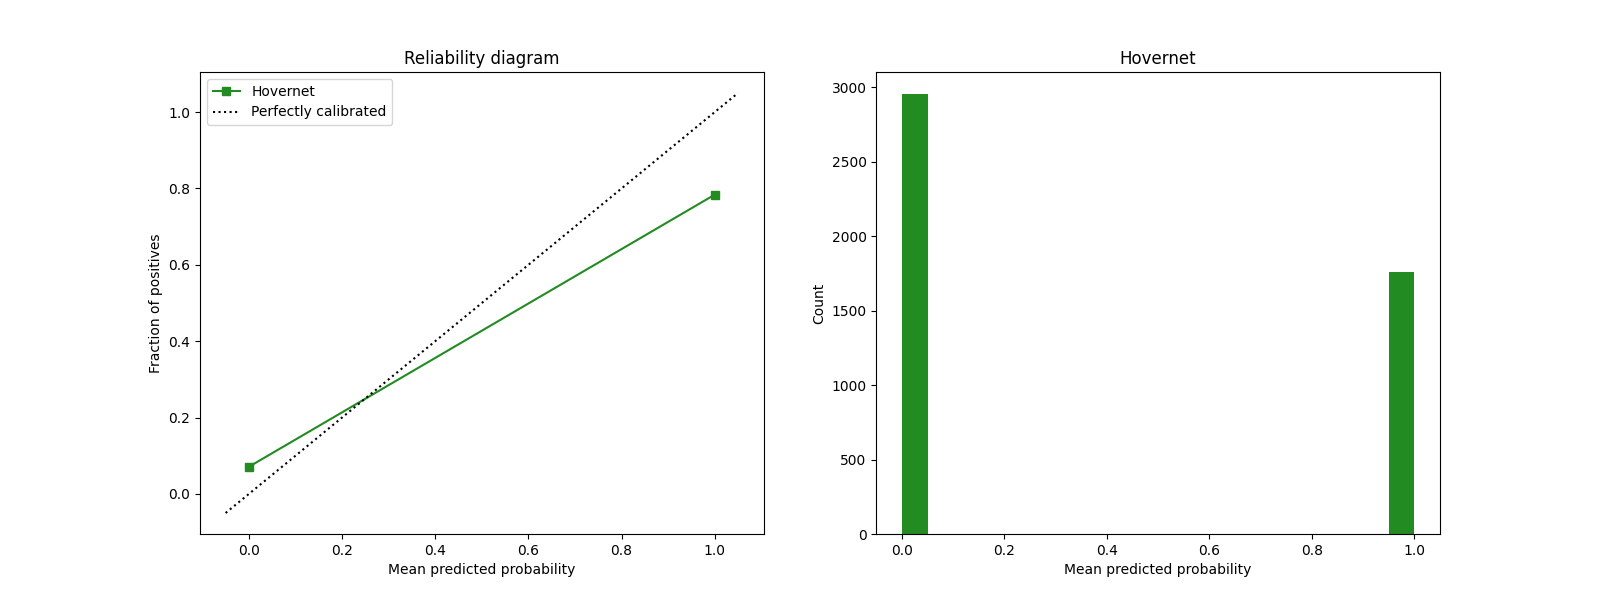
\includegraphics[width=\textwidth]{imgs/hov_rel_diag.png}
    \caption{Reliability diagram of Hovernet from one of our experiments. At the right is the histogram of the predicted probabilities, clearly not a uniform distribution.}
    \label{fig:hov_rel}
\end{figure}

Reliability diagrams can be converted into a metric in the same way the ROC was made a metric by using the area under it. Here, instead of the area under the curve, the area between the model curve and a perfectly calibrated curve is taken. Furthermore, since points in that diagram can represent sets of arbitrary size the area of each bin is weighted by the number of samples in it. Where now we are calling the points bins, since in fact, each point has a width that represents the range of probabilities it takes into account. A more appropriate visualisation is on \autoref{fig:rel2}. The metric derived is called Expected Calibration Error (ECE).

\begin{figure}[ht]
    \centering
    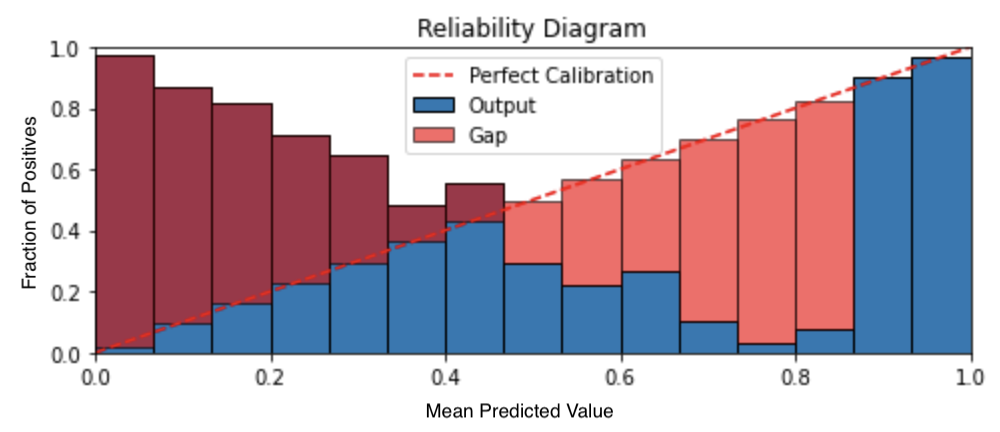
\includegraphics[width=\textwidth]{imgs/rel2.png}
    \caption{Another way of representing a reliability diagram.}
    \label{fig:rel2}
\end{figure}

\subsection{Extending metrics}

I have depicted a clear way of measuring uncertainty calibration in the previous section but it has at least one downside, it is only for binary problems. I'll devote this subsection to a way in which one can extend any binary metric to a multiclass metric. Suppose we have a metric called $M$.  Now, given a multiclass setup one can compute $M^k$, the same metric but considering the class $k$ against the others. By grouping all the other classes into one, the problem is now binary and so we can compute $M$. By averaging all the $M^k$ we get the extension of $M$. For instance, the macro $F_1$ score correspond to doing this to the $F_1$ score with equal weights to all classes. While the weighted $F_1$ score is the weighted average of the individual $F_1$ scores. However, the micro $F_1$ score, which is also called accuracy, does not correspond to the extension of the accuracy, although it is quite close. The extension of the accuracy is in fact $\frac{2}{N} \text{Micro} + \frac{N-2}{N}$ being $N$ the number of classes. The proof is straightforward. If we call $D$ the diagonal of the confusion matrix and $T$ the total sum then

\begin{align}
    Acc^k &= \frac{a_{kk} + \sum_{i,j \neq k} a_{ij}}{\sum_{i,j}a_{ij}} \\
    Acc_{extended} &= \frac{1}{N} \sum_{k} Acc^k = \frac{\sum_{k}a_{kk} + \sum_{k} \sum_{i,j\neq k} a_{ij}}{N \sum_{i,j}a_{ij}} \\
    &= \frac{2D + (N-2) T}{N T} = \frac{2}{N} \text{Micro} + \frac{N-2}{N}
\end{align}

where the intermediate step can be deduced by counting how many times does each term appears. The diagonal terms appear $N-1$ times while the rest of terms appear $N-2$ times, therefore $\sum_{k} \sum_{i,j\neq k} a_{ij} = D + (N-1)T$, concluding the proof. Surprisingly enough, the extension of the accuracy approaches 1 as the number of classes increases so it is quite a bad metric. In the experiments below, we will be using the extension of the ECE and call it just ECE for simplicity in the multiclass datasets.

\section{Experiments}\label{sec:exp}

Two experiments were carried out to show the usefulness of graph neural networks in the problem of cell detection and another two experiments were made to provide insights about the models involved. Results are in \autoref{sec:results}, this section is only to describe the experiments themselves. 


\subsection{GNN vs CNN}

The main experiment and the one that supports the principal thesis of this work compares convolutional neural networks with graph neural networks. In order to state that GNNs are actually useful they must outperform CNNs (Hovernet) in every metric defined in \autoref{sec:metrics}. But outperforming in just one dataset is not enough. For that reason the comparison will be made using all the datasets from the original Hovernet article \cite{hovernet, gamper2020pannuke, 8880654}, and using several internal datasets of the DigiPatics project \cite{DigiPatics2022}. More concretely, the methods will be evaluated in the HER2 stained breast dataset and the H\&E stained lung dataset. For the multi-class problems, multi-class metrics will be taken into account and for binary problems, binary metrics.

\subsection{GNN vs XGBoost}

Outperforming CNNs may not be due to the graph structure. It is possible that the extracted features are sufficient to improve CNN results. It may be that the edges do not contain any useful information. To account for that, GNN must be compared with node-only methods. In this case we selected XGBoost \cite{xgboost} for comparison since it has been in the leaderboard of several Kaggle competitions\footnote{\url{https://dataaspirant.com/xgboost-algorithm/}}. By comparing node-only methods with GNNs we can know if the value of GNNs reside on the extracted features or on the graph structure itself.

\subsection{Scaling CNNs}

The original Hovernet article restricted their images to having 270x270 pixels. That is a very narrow view of the cells. It seems intuitive that increasing the receptive field of the model increases its performance too. But science does not understand intuition, only facts. So an experiment needs to be carried out in order to prove if increasing the receptive field is really beneficial. Apart from that, since the original weights of Hovernet are open source, we can initialise our weights with them. Therefore, there are four different models that we will call 270, 270FT, 518 and 518FT. The number indicates the resolution of the images and FT means fine-tuned. The models with FT in the name initialise their weights with the ones from the original Hovernet article. The other models initialise their weights at random. The datasets used in this experiment are only our own lung and breast datasets.

\subsection{Void GNNs}

Finally, the last experiment is about knowing if the extracted features are relevant or not. We distinguish two types of features: morphological and probabilities. The first group is independent from the Hovernet output while the second is not. To see which of them are more important we train the same GNN models with different features. One with all the features, one only with morphological features and another only with probabilities. By comparing the metrics obtained we can discern which set of features is more relevant.
